\section{Auswertung}
\subsection{Getestete Szenen}
\begin{figure}
  \center
  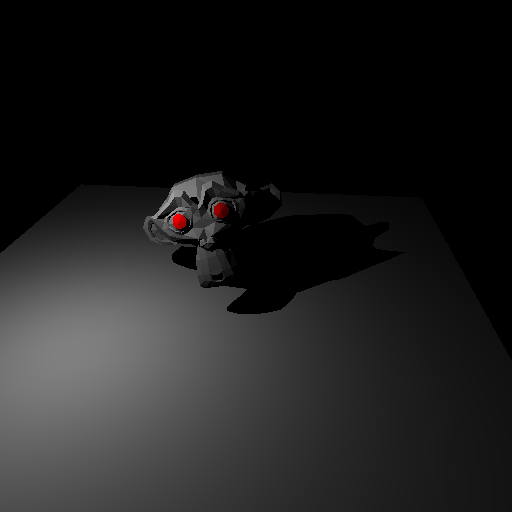
\includegraphics[width=.6\textwidth]{images/monkey.png}
  \caption{Monkey Szene}
\end{figure}
\begin{figure}
  \center
  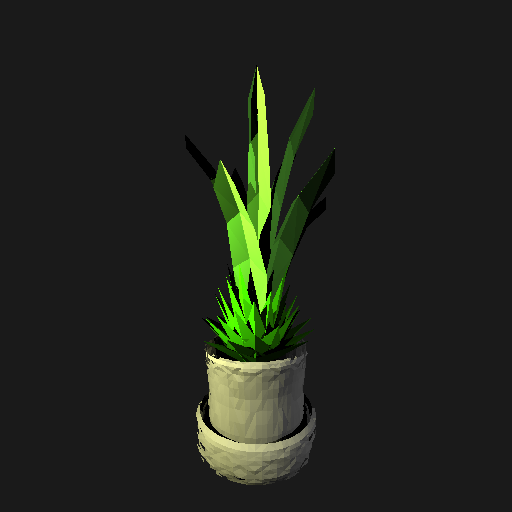
\includegraphics[width=.6\textwidth]{images/plant.png}
 \caption{Plant Szene}
\end{figure}
\begin{figure}
  \center
  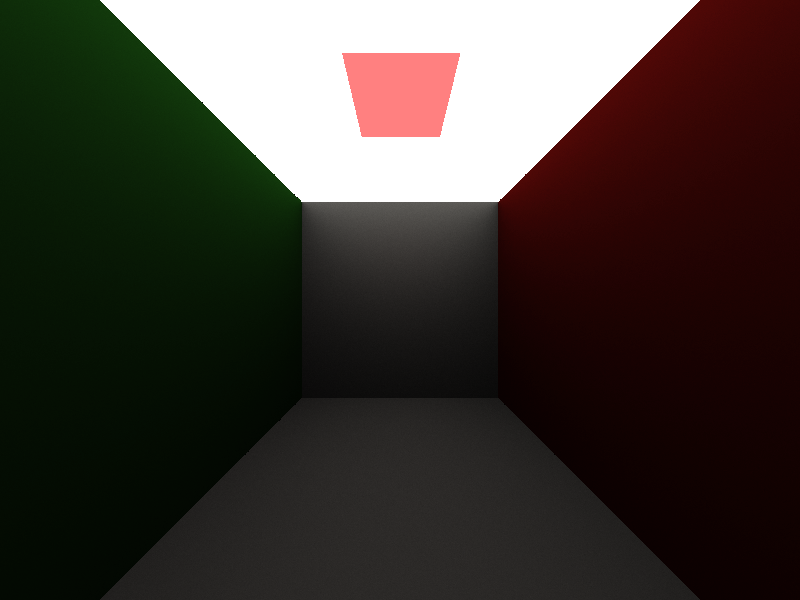
\includegraphics[width=.6\textwidth]{images/pt_cornell.png}
  \caption{PT/Cornell Szene}
\end{figure}
  
\subsection{Getestete Konfigurationen}
\subsection{Ergebnisse}
\begin{figure}
  \center
  \caption{Monkey Szene}
  \label{fig:runtime_monkey}
  \begin{tikzpicture}
  \begin{axis} [
    symbolic x coords={Baseline,Adaptive-Sampling,OpenMP,SSERay,BIH,KdTree,Kombiniert},
    table/header=false,
    enlargelimits=0.15,
    ymode=log,
    scaled y ticks = false,
    ylabel={Laufzeit (ms)},
    xtick=data,
    x tick label style={rotate=45,anchor=east},
  ]
      \addplot [box plot median] table {evaluation/monkey.dat};
      \addplot [box plot box] table {evaluation/monkey.dat};
      \addplot [box plot top whisker] table {evaluation/monkey.dat};
      \addplot [box plot bottom whisker] table {evaluation/monkey.dat};
  \end{axis}
  \end{tikzpicture}
\end{figure}

\begin{figure}
  \center
  \caption{Plant Szene}
  \label{fig:runtime_plant}
  \begin{tikzpicture}
  \begin{axis} [
    symbolic x coords={Baseline,Adaptive-Sampling,OpenMP,SSERay,BIH,KdTree,Kombiniert},
    table/header=false,
    enlargelimits=0.15,
    ymode=log,
    scaled y ticks = false,
    ylabel={Laufzeit (ms)},
    xtick=data,
    x tick label style={rotate=45,anchor=east},
  ]
      \addplot [box plot median] table {evaluation/plant.dat};
      \addplot [box plot box] table {evaluation/plant.dat};
      \addplot [box plot top whisker] table {evaluation/plant.dat};
      \addplot [box plot bottom whisker] table {evaluation/plant.dat};
  \end{axis}
  \end{tikzpicture}
\end{figure}

\begin{figure}
  \center
  \caption{PT/Cornell Szene}
  \label{fig:runtime_pt_cornell}
  \begin{tikzpicture}
  \begin{axis} [
    symbolic x coords={Baseline,Adaptive-Sampling,OpenMP,SSERay,Cuda,BIH,KdTree,Kombiniert},
    table/header=false,
    enlargelimits=0.15,
    ymode=log,
    scaled y ticks = false,
    ylabel={Laufzeit (ms)},
    xtick=data,
    x tick label style={rotate=45,anchor=east},
  ]
      \addplot [box plot median] table {evaluation/pt_cornell.dat};
      \addplot [box plot box] table {evaluation/pt_cornell.dat};
      \addplot [box plot top whisker] table {evaluation/pt_cornell.dat};
      \addplot [box plot bottom whisker] table {evaluation/pt_cornell.dat};
  \end{axis}
  \end{tikzpicture}
\end{figure}
